\documentclass{article}

% If you're new to LaTeX, here's some short tutorials:
% https://www.overleaf.com/learn/latex/Learn_LaTeX_in_30_minutes
% https://en.wikibooks.org/wiki/LaTeX/Basics

% Formatting
\usepackage[utf8]{inputenc}
\usepackage[margin=1in]{geometry}

% Math
% https://www.overleaf.com/learn/latex/Mathematical_expressions
% https://en.wikibooks.org/wiki/LaTeX/Mathematics
\usepackage{amsmath,amsfonts,amssymb,mathtools}

% Images
% https://www.overleaf.com/learn/latex/Inserting_Images
% https://en.wikibooks.org/wiki/LaTeX/Floats,_Figures_and_Captions
\usepackage{graphicx,float}

% Tables
% https://www.overleaf.com/learn/latex/Tables
% https://en.wikibooks.org/wiki/LaTeX/Tables

% Algorithms
% https://www.overleaf.com/learn/latex/algorithms
% https://en.wikibooks.org/wiki/LaTeX/Algorithms
\usepackage[ruled,vlined]{algorithm2e}
\usepackage{algorithmic}

% Code syntax highlighting
% https://www.overleaf.com/learn/latex/Code_Highlighting_with_minted
\usepackage{minted}
\usemintedstyle{borland}


\usepackage{tikz}
\usetikzlibrary{positioning}

% Title content
\title{CS264A Homework 1}
\author{Bobby Judd}
\date{October 21, 2020}

\begin{document}

\maketitle

% 1
\noindent\rule{16cm}{0.4pt}
\section{}
\begin{itemize}
\item $(\lnot A \implies B) \land (A \implies \lnot B) = (A \lor B) \land (\lnot A \lor \lnot B)$
\item $(A \land B) \implies (\lnot A \lor \lnot B) = \lnot(A \lor B) \lor (\lnot A \lor \lnot B)$
\end{itemize}
The world where \textbf{A = true} and \textbf{B = false}, satisfies each sentence:
\begin{itemize}
\item $(true \lor false) \land (\lnot true \lor \lnot false) = true \land true = true$
\item $\lnot(true \lor false) \lor (\lnot true \lor \lnot false) = false \lor true = true$
\end{itemize}

% 2 
\noindent\rule{16cm}{0.4pt}
\section{}
\begin{itemize}
\item $(A \implies B) \implies (\lnot B \implies \lnot A)\\
       = \lnot(\lnot A \lor B) \lor (B \lor \lnot A)\\
       = (A \land \lnot B) \lor (B \lor \lnot A)\\
       = (A \land \lnot B) \lor \lnot (A \land \lnot B)\\
       = true$
\item $((A \lor B) \land (A \implies C)) \implies (B \lor C)\\
        = \lnot ((A \lor B) \land (\lnot A \lor C)) \lor (B \lor C)\\
        = \lnot(B \lor C) \lor (B \lor C)\\
        = true$
\end{itemize}
The reduction of both sentences yields \textbf{true} indicating both are \textbf{true} at every world and thus both are \textbf{valid}.

% 3
\noindent\rule{16cm}{0.4pt}
\section{}
\renewcommand{\labelenumi}{(\alph{enumi})}
 \begin{enumerate}
   \item $\exists P (\Delta) \lor \exists P (\Gamma) \\
   = \Delta | P \lor \Delta | \lnot P \lor \Gamma | P \lor \Gamma | \lnot P \\
   = (\Delta | P \lor \Gamma | P) \lor (\Delta | \lnot P \lor \Gamma | \lnot P) \quad \textrm{associative prop.}\\
   = (\Delta \lor \Gamma) | P \lor (\Delta \lor \Gamma) | \lnot P \\
   = \exists P (\Delta \lor \Gamma) $
   \item $ (\forall P \Delta) \land (\forall P \Gamma) \\
   = \Delta | P \land \Delta | \lnot P \land \Gamma | P \land \Gamma | \lnot P \\
   = (\Delta | P \land \Gamma | P) \land (\Delta | \lnot P \land \Gamma | \lnot P) \quad \textrm{associative prop.}\\
   = (\Delta \land \Gamma) | P \land (\Delta \land \Gamma) | \lnot P$
 \end{enumerate}

 % 4
 \noindent\rule{16cm}{0.4pt}
 \section{}
 \[\Delta = A \Rightarrow B, \lnot A \Rightarrow (\lnot B \land C), (B \lor C) \Rightarrow D\]
 \[= \lnot A \lor B, \quad A \lor (\lnot B \land C), \quad (\lnot B \land \lnot C) \lor D\]
 \[= \lnot A \lor B, \quad (A \lor \lnot B) \land (A \lor C), \quad (\lnot B \lor D) \land (\lnot C \lor D)\]
 \[= \lnot A \lor B, \quad (A \lor \lnot B), (A \lor C), \quad (\lnot B \lor D), (\lnot C \lor D)\]
 \[= \{\{\lnot A, B\}, \quad \{A, \lnot B\}, \quad \{A, C\}, \quad \{\lnot B, D\}, \quad \{\lnot C, D\}\}\]
 
 % 5
 \noindent\rule{16cm}{0.4pt}
 \section{}
 Mods(KB) = Models of KB \\
 CE(KB) = Clausal Entailment of KB\\
 \begin{center}
 The equivalence of two KB's $\Gamma$ and $\Delta$ is true if:\\
 $CE(\Gamma \land \lnot \Delta) = \{\emptyset\}$ AND $Mods(\Gamma \land \lnot \Delta) = \emptyset$
 \end{center}
 
 Each polynomial procedure would be run once. The production of the KB $\Gamma \land \lnot \Delta$ would only be a linear procedure which would ultimately yield a polynomial procedure for equivalence.
 
 % 6
 \noindent\rule{16cm}{0.4pt}
 \section{}
 \[\Delta = \{\{A, B\}, \{\lnot A, \lnot C\}, \{D, \lnot B \}, \{D, \lnot C \}, \{\lnot A, E\}\}\]
  \renewcommand{\labelenumi}{\arabic{enumi}.}
 \begin{enumerate}
 \item $\{A, B\}$
 \item $\{\lnot A, \lnot C\}$
 \item $\{D, \lnot B \}$
 \item $\{D, \lnot C \}$
 \item $\{\lnot A, E \}$
 \newline
 \noindent\rule{4cm}{0.4pt}
 \item $\{B, E \}$ \quad Resolving A over 1 \& 5
 \item $\{D, E \}$ \quad Resolving B over 3 \& 6
 \end{enumerate}
 
 % 7
 \noindent\rule{16cm}{0.4pt}
 \section{}
 \[\Delta = (\lnot A \lor \lnot D \lor E) \land
            (\lnot C \lor D) \land
            (\lnot D \lor \lnot E) \land
            (\lnot B \lor C \lor D) \]
\[  \quad = \{\{\lnot A, \lnot D, E\},
            \{\lnot C, D\},
            \{\lnot D, \lnot E\},
            \{\lnot B, C, D\}\} \]
\newline
\newline
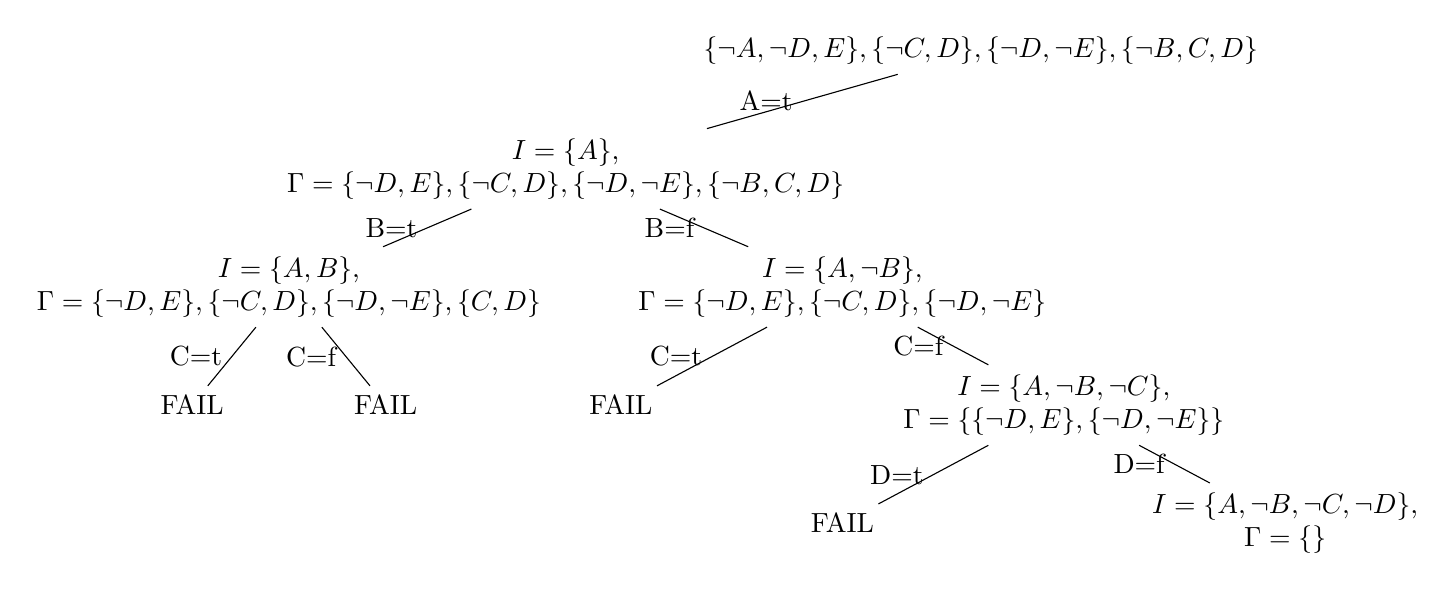
\begin{tikzpicture}
\node {$\{\lnot A, \lnot D, E\},
            \{\lnot C, D\},
            \{\lnot D, \lnot E\},
            \{\lnot B, C, D\}$}[sibling distance=30em, align=center]
    child {node {$I = \{A\}$,\\ $\Gamma = \{\lnot D, E\},
            \{\lnot C, D\},
            \{\lnot D, \lnot E\},
            \{\lnot B, C, D\}$}[sibling distance=20em]
                child {
                node {$I = \{A, B\}$,\\ $\Gamma = \{\lnot D, E\},
                \{\lnot C, D\},
                \{\lnot D, \lnot E\},
                \{C, D\}$} [sibling distance=7em]
                    child {
                    node {FAIL}
                    edge from parent node[left]{C=t}
                    }
                    child {
                    node {FAIL}
                    edge from parent node[left]{C=f}
                    }
                edge from parent node[left]{B=t}
                }
                child {
                node {$I = \{A, \lnot B\}$,\\ $\Gamma = \{\lnot D, E\},
                \{\lnot C, D\},
                \{\lnot D, \lnot E\}$} [sibling distance=16em]
                    child {
                    node {FAIL}
                    edge from parent node[left]{C=t}
                    }
                    child {
                    node {$I = \{A, \lnot B, \lnot C\}$,\\ $\Gamma = \{\{\lnot D, E\},\{\lnot D, \lnot E\}\}$}
                        child {
                        node {FAIL}
                        edge from parent node[left]{D=t}
                        }
                        child {
                        node {$I = \{A, \lnot B, \lnot C, \lnot D\}$,\\ $\Gamma = \{\}$}
                        edge from parent node[left]{D=f}
                        }
                    edge from parent node[left]{C=f}
                    }
                edge from parent node[left]{B=f}
                }
            edge from parent node[left]{A=t}
            }
            child{edge from parent[draw=none]};
\end{tikzpicture}

% 8
\noindent\rule{16cm}{0.4pt}
\section{}
See attached for written submission.

% 9
\noindent\rule{16cm}{0.4pt}
\section{}
\[\Delta = (\lnot A \lor B) \land
            (A \lor \lnot B) \land
            (A \lor C) \land
            (D \lor \lnot B) \land
            (D \lor \lnot C) \]
\[\quad =  \{\{\lnot A , B\} ,
            \{A , \lnot B\} ,
            \{A , C\} ,
            \{D , \lnot B\} ,
            \{D , \lnot C\}\} \]
\newline
\begin{center}
CDPLL
\end{center}
\begin{center}
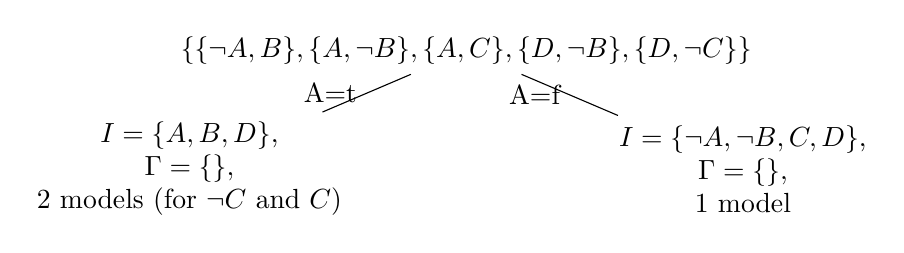
\begin{tikzpicture}
\node {$\{\{\lnot A , B\} ,
            \{A , \lnot B\} ,
            \{A , C\} ,
            \{D , \lnot B\} ,
            \{D , \lnot C\}\}$}[sibling distance=20em, align=center]
    child {
            node {
                $I = \{A, B, D\}$,\\
                $\Gamma = \{\},$ \\
                2 models (for $\lnot C$ and $C$)
            }
            edge from parent node[left]{A=t}
    }
    child {
        node {
            $I = \{\lnot A, \lnot B, C, D\}$,\\
            $\Gamma = \{\},$ \\
            1 model
        }
        edge from parent node[left]{A=f}
    };
\end{tikzpicture}
\newline
$\Delta$ contains 3 models, which are obtained by counting the models in each leaf node.
\end{center}

% 10
\noindent\rule{16cm}{0.4pt}
\section{}
\renewcommand{\labelenumi}{(\alph{enumi})}
 \begin{enumerate}
   \item $\Delta = \{\{P_1, P_2, P_3\}, \{\lnot P_1, Q\}, \{\lnot P_3, Q\}\}$
   \item
        \begin{itemize}
            \item $P_1$: $\{P_2, P_3, Q\}$ Using 1 and 2
            \item $P_2$: No legitimate resolutions
            \item $P_3$: No legitimate resolutions
            \item $Q$: No legitimate resolutions
        \end{itemize}
   \item Decision Tree:\newline
   \begin{tikzpicture}
    \node {$P_1$}[sibling distance=16em, align=center]
        child {
                node {$P_2$}[sibling distance=8em]
                child {
                    node {$P_3$}[sibling distance=4em]
                    child {
                        node {$Q$}[sibling distance=2em]
                        child {
                            node {T} edge from parent [solid]
                        }
                        child {
                            node {F} edge from parent [dashed]
                        }
                        edge from parent [solid]
                    }
                    child {
                        node {$Q$}[sibling distance=2em]
                        child {
                            node {T} edge from parent [solid]
                        }
                        child {
                            node {F} edge from parent [dashed]
                        }
                        edge from parent [dashed]
                    }
                    edge from parent [solid]
                }
                child {
                    node {$P_3$}[sibling distance=4em]
                    child {
                        node {$Q$}[sibling distance=2em]
                        child {
                            node {T} edge from parent [solid]
                        }
                        child {
                            node {F} edge from parent [dashed]
                        }
                        edge from parent [solid]
                    }
                    child {
                        node {$Q$}[sibling distance=2em]
                        child {
                            node {T} edge from parent [solid]
                        }
                        child {
                            node {F} edge from parent [dashed]
                        }
                        edge from parent [dashed]
                    }
                    edge from parent [dashed]
                }
                edge from parent [solid]
        }
        child {
                node {$P_2$}[sibling distance=8em]
                child {
                    node {$P_3$}[sibling distance=4em]
                    child {
                        node {$Q$}[sibling distance=2em]
                        child {
                            node {T} edge from parent [solid]
                        }
                        child {
                            node {F} edge from parent [dashed]
                        }
                        edge from parent [solid]
                    }
                    child {
                        node {$Q$}[sibling distance=2em]
                        child {
                            node {T} edge from parent [solid]
                        }
                        child {
                            node {T} edge from parent [dashed]
                        }
                        edge from parent [dashed]
                    }
                    edge from parent [solid]
                }
                child {
                    node {$P_3$}[sibling distance=4em]
                    child {
                        node {$Q$}[sibling distance=2em]
                        child {
                            node {T} edge from parent [solid]
                        }
                        child {
                            node {F} edge from parent [dashed]
                        }
                        edge from parent [solid]
                    }
                    child {
                        node {$Q$}[sibling distance=2em]
                        child {
                            node {F} edge from parent [solid]
                        }
                        child {
                            node {F} edge from parent [dashed]
                        }
                        edge from parent [dashed]
                    }
                    edge from parent [dashed]
                }
                edge from parent [dashed]
        };
    \end{tikzpicture}
\newline
$\Delta$ contains 8 models, which are obtained by counting the "T" leaf nodes.
 \end{enumerate}

\end{document}